% Options for packages loaded elsewhere
\PassOptionsToPackage{unicode}{hyperref}
\PassOptionsToPackage{hyphens}{url}
\PassOptionsToPackage{dvipsnames,svgnames,x11names}{xcolor}
%
\documentclass[
  letterpaper,
  DIV=11,
  numbers=noendperiod]{scrartcl}

\usepackage{amsmath,amssymb}
\usepackage{iftex}
\ifPDFTeX
  \usepackage[T1]{fontenc}
  \usepackage[utf8]{inputenc}
  \usepackage{textcomp} % provide euro and other symbols
\else % if luatex or xetex
  \usepackage{unicode-math}
  \defaultfontfeatures{Scale=MatchLowercase}
  \defaultfontfeatures[\rmfamily]{Ligatures=TeX,Scale=1}
\fi
\usepackage{lmodern}
\ifPDFTeX\else  
    % xetex/luatex font selection
\fi
% Use upquote if available, for straight quotes in verbatim environments
\IfFileExists{upquote.sty}{\usepackage{upquote}}{}
\IfFileExists{microtype.sty}{% use microtype if available
  \usepackage[]{microtype}
  \UseMicrotypeSet[protrusion]{basicmath} % disable protrusion for tt fonts
}{}
\makeatletter
\@ifundefined{KOMAClassName}{% if non-KOMA class
  \IfFileExists{parskip.sty}{%
    \usepackage{parskip}
  }{% else
    \setlength{\parindent}{0pt}
    \setlength{\parskip}{6pt plus 2pt minus 1pt}}
}{% if KOMA class
  \KOMAoptions{parskip=half}}
\makeatother
\usepackage{xcolor}
\setlength{\emergencystretch}{3em} % prevent overfull lines
\setcounter{secnumdepth}{-\maxdimen} % remove section numbering
% Make \paragraph and \subparagraph free-standing
\ifx\paragraph\undefined\else
  \let\oldparagraph\paragraph
  \renewcommand{\paragraph}[1]{\oldparagraph{#1}\mbox{}}
\fi
\ifx\subparagraph\undefined\else
  \let\oldsubparagraph\subparagraph
  \renewcommand{\subparagraph}[1]{\oldsubparagraph{#1}\mbox{}}
\fi

\usepackage{color}
\usepackage{fancyvrb}
\newcommand{\VerbBar}{|}
\newcommand{\VERB}{\Verb[commandchars=\\\{\}]}
\DefineVerbatimEnvironment{Highlighting}{Verbatim}{commandchars=\\\{\}}
% Add ',fontsize=\small' for more characters per line
\usepackage{framed}
\definecolor{shadecolor}{RGB}{241,243,245}
\newenvironment{Shaded}{\begin{snugshade}}{\end{snugshade}}
\newcommand{\AlertTok}[1]{\textcolor[rgb]{0.68,0.00,0.00}{#1}}
\newcommand{\AnnotationTok}[1]{\textcolor[rgb]{0.37,0.37,0.37}{#1}}
\newcommand{\AttributeTok}[1]{\textcolor[rgb]{0.40,0.45,0.13}{#1}}
\newcommand{\BaseNTok}[1]{\textcolor[rgb]{0.68,0.00,0.00}{#1}}
\newcommand{\BuiltInTok}[1]{\textcolor[rgb]{0.00,0.23,0.31}{#1}}
\newcommand{\CharTok}[1]{\textcolor[rgb]{0.13,0.47,0.30}{#1}}
\newcommand{\CommentTok}[1]{\textcolor[rgb]{0.37,0.37,0.37}{#1}}
\newcommand{\CommentVarTok}[1]{\textcolor[rgb]{0.37,0.37,0.37}{\textit{#1}}}
\newcommand{\ConstantTok}[1]{\textcolor[rgb]{0.56,0.35,0.01}{#1}}
\newcommand{\ControlFlowTok}[1]{\textcolor[rgb]{0.00,0.23,0.31}{#1}}
\newcommand{\DataTypeTok}[1]{\textcolor[rgb]{0.68,0.00,0.00}{#1}}
\newcommand{\DecValTok}[1]{\textcolor[rgb]{0.68,0.00,0.00}{#1}}
\newcommand{\DocumentationTok}[1]{\textcolor[rgb]{0.37,0.37,0.37}{\textit{#1}}}
\newcommand{\ErrorTok}[1]{\textcolor[rgb]{0.68,0.00,0.00}{#1}}
\newcommand{\ExtensionTok}[1]{\textcolor[rgb]{0.00,0.23,0.31}{#1}}
\newcommand{\FloatTok}[1]{\textcolor[rgb]{0.68,0.00,0.00}{#1}}
\newcommand{\FunctionTok}[1]{\textcolor[rgb]{0.28,0.35,0.67}{#1}}
\newcommand{\ImportTok}[1]{\textcolor[rgb]{0.00,0.46,0.62}{#1}}
\newcommand{\InformationTok}[1]{\textcolor[rgb]{0.37,0.37,0.37}{#1}}
\newcommand{\KeywordTok}[1]{\textcolor[rgb]{0.00,0.23,0.31}{#1}}
\newcommand{\NormalTok}[1]{\textcolor[rgb]{0.00,0.23,0.31}{#1}}
\newcommand{\OperatorTok}[1]{\textcolor[rgb]{0.37,0.37,0.37}{#1}}
\newcommand{\OtherTok}[1]{\textcolor[rgb]{0.00,0.23,0.31}{#1}}
\newcommand{\PreprocessorTok}[1]{\textcolor[rgb]{0.68,0.00,0.00}{#1}}
\newcommand{\RegionMarkerTok}[1]{\textcolor[rgb]{0.00,0.23,0.31}{#1}}
\newcommand{\SpecialCharTok}[1]{\textcolor[rgb]{0.37,0.37,0.37}{#1}}
\newcommand{\SpecialStringTok}[1]{\textcolor[rgb]{0.13,0.47,0.30}{#1}}
\newcommand{\StringTok}[1]{\textcolor[rgb]{0.13,0.47,0.30}{#1}}
\newcommand{\VariableTok}[1]{\textcolor[rgb]{0.07,0.07,0.07}{#1}}
\newcommand{\VerbatimStringTok}[1]{\textcolor[rgb]{0.13,0.47,0.30}{#1}}
\newcommand{\WarningTok}[1]{\textcolor[rgb]{0.37,0.37,0.37}{\textit{#1}}}

\providecommand{\tightlist}{%
  \setlength{\itemsep}{0pt}\setlength{\parskip}{0pt}}\usepackage{longtable,booktabs,array}
\usepackage{calc} % for calculating minipage widths
% Correct order of tables after \paragraph or \subparagraph
\usepackage{etoolbox}
\makeatletter
\patchcmd\longtable{\par}{\if@noskipsec\mbox{}\fi\par}{}{}
\makeatother
% Allow footnotes in longtable head/foot
\IfFileExists{footnotehyper.sty}{\usepackage{footnotehyper}}{\usepackage{footnote}}
\makesavenoteenv{longtable}
\usepackage{graphicx}
\makeatletter
\def\maxwidth{\ifdim\Gin@nat@width>\linewidth\linewidth\else\Gin@nat@width\fi}
\def\maxheight{\ifdim\Gin@nat@height>\textheight\textheight\else\Gin@nat@height\fi}
\makeatother
% Scale images if necessary, so that they will not overflow the page
% margins by default, and it is still possible to overwrite the defaults
% using explicit options in \includegraphics[width, height, ...]{}
\setkeys{Gin}{width=\maxwidth,height=\maxheight,keepaspectratio}
% Set default figure placement to htbp
\makeatletter
\def\fps@figure{htbp}
\makeatother

\KOMAoption{captions}{tableheading}
\makeatletter
\@ifpackageloaded{caption}{}{\usepackage{caption}}
\AtBeginDocument{%
\ifdefined\contentsname
  \renewcommand*\contentsname{Table of contents}
\else
  \newcommand\contentsname{Table of contents}
\fi
\ifdefined\listfigurename
  \renewcommand*\listfigurename{List of Figures}
\else
  \newcommand\listfigurename{List of Figures}
\fi
\ifdefined\listtablename
  \renewcommand*\listtablename{List of Tables}
\else
  \newcommand\listtablename{List of Tables}
\fi
\ifdefined\figurename
  \renewcommand*\figurename{Figure}
\else
  \newcommand\figurename{Figure}
\fi
\ifdefined\tablename
  \renewcommand*\tablename{Table}
\else
  \newcommand\tablename{Table}
\fi
}
\@ifpackageloaded{float}{}{\usepackage{float}}
\floatstyle{ruled}
\@ifundefined{c@chapter}{\newfloat{codelisting}{h}{lop}}{\newfloat{codelisting}{h}{lop}[chapter]}
\floatname{codelisting}{Listing}
\newcommand*\listoflistings{\listof{codelisting}{List of Listings}}
\makeatother
\makeatletter
\makeatother
\makeatletter
\@ifpackageloaded{caption}{}{\usepackage{caption}}
\@ifpackageloaded{subcaption}{}{\usepackage{subcaption}}
\makeatother
\ifLuaTeX
  \usepackage{selnolig}  % disable illegal ligatures
\fi
\IfFileExists{bookmark.sty}{\usepackage{bookmark}}{\usepackage{hyperref}}
\IfFileExists{xurl.sty}{\usepackage{xurl}}{} % add URL line breaks if available
\urlstyle{same} % disable monospaced font for URLs
\hypersetup{
  pdftitle={Regression Discontinuity Design},
  pdfauthor={Fernando Rios-Avila},
  colorlinks=true,
  linkcolor={blue},
  filecolor={Maroon},
  citecolor={Blue},
  urlcolor={Blue},
  pdfcreator={LaTeX via pandoc}}

\title{Regression Discontinuity Design}
\usepackage{etoolbox}
\makeatletter
\providecommand{\subtitle}[1]{% add subtitle to \maketitle
  \apptocmd{\@title}{\par {\large #1 \par}}{}{}
}
\makeatother
\subtitle{Up close, we are all the same}
\author{Fernando Rios-Avila}
\date{}

\begin{document}
\maketitle
\subsection{Re-Cap: Potential outcome
Model}\label{re-cap-potential-outcome-model}

In the ideal world, where we can see all possible outcomes and scenarios
of your potential treatments, it will be very simple to estimate
treatment effects:

\[
\delta_i = Y_i(1)-Y_i(0)
\]

This works because all observed and unobserved individual
characteristics are kept fixed, except for the treatment Status.

\[y_i(D)=y_i(X,u,D)\]

So when comparing a person with himself (clones or parallel worlds), we
know (or at least expect) that everything else is the same, and that
differences between the two states are explained only by the treatment.

\subsection{The Problem}\label{the-problem}

We do not observe both \textbf{ALL} States at the same time. People will
either be treated or untreated, not both.

So what can we do?

\begin{quote}
\textbf{We need to find good counterfactuals!}
\end{quote}

This means finding people are very similar to the ones treated, so they
can be used as the examples of the ``what if'' question.

But there is a problem. Even in the best scenarios, we can never be
asure about how to control for unobservables\ldots or can we?

\subsection{}\label{section}

\begin{itemize}
\item
  \textbf{You can always RCT} But it can be expensive
\item
  \textbf{You can IV the problem} but its hard to justify
\item
  \textbf{You can add FE}, but you have time varying errors
\end{itemize}

Then what?

\begin{itemize}
\tightlist
\item
  You could RDD the problem (if you have the right data!)
\end{itemize}

\subsection{What is RDD?}\label{what-is-rdd}

\textbf{RDD} or Regression Discontinuity design is methodology that is
known for its clean identification and with a relatively easy
visualization tool to understand the identification, and solve the
problem of unobserved distributions. (see
\href{https://academic.oup.com/qje/advance-article/doi/10.1093/qje/qjad011/7068116?login=true}{here}
for a recent paper on how to make graphs on this).

In fact, the treatment Status has a very clear Rule!

Consider the following problem:

\begin{enumerate}
\def\labelenumi{\arabic{enumi}.}
\tightlist
\item
  You want to study the role of college on earnings.
\item
  You have data on people who are applying to go to school. They all
  take some standardized tests. Their grade will determine if they get
  into College or not.
\item
  People with high skills will get a higher grades in the GRE, go to
  college, and probably get higher salaries.
\item
  But, there is a problem. How can you figure out if wages are due to
  College or skill?
\end{enumerate}

\subsection{Possible Solution}\label{possible-solution}

Say that we actually have access to the grades, which range from 100 to
200. And assume that you say, every one with grades higher than 170 will
go to college.

Can you estimate the effect now?

\begin{itemize}
\tightlist
\item
  You can't compare people with more than 170 to those with less than
  170. Because skill or ability will be different across groups.
\item
  However, what if you compare individuals with 170-172 vs 167-169?

  \begin{itemize}
  \tightlist
  \item
    These individuals are so close togeter they problably have very
    similar characteristics as well!
  \item
    you have a Localized randomization.
  \end{itemize}
\end{itemize}

In this case, your analysis is those individuals just above the
thresholds to those just below (counterfactual)

Unless you think grades near the threshold are as good as random, then
you have a design to identify treatment effects!

\subsection{RDD: How it works.}\label{rdd-how-it-works.}

\textbf{Selection and Index}:

\begin{enumerate}
\def\labelenumi{\arabic{enumi}.}
\tightlist
\item
  The first thing you need to see if you can use and RDD is to see if
  you have access to a variable that ``ranks'' units.
\end{enumerate}

\begin{itemize}
\tightlist
\item
  This variable should be smooth and preferibly continuous.

  \begin{itemize}
  \tightlist
  \item
    age, distance from boarder, test score, poverty index
  \end{itemize}
\end{itemize}

\begin{enumerate}
\def\labelenumi{\arabic{enumi}.}
\setcounter{enumi}{1}
\tightlist
\item
  Assignment into treatment is a function of this index only, with a
  clear threshold for the index to have an impact the treatment.
\end{enumerate}

\begin{itemize}
\tightlist
\item
  Those under the Threshold are not treated. Those above are.
\item
  This is called a \textbf{Sharp RDD} design.
\end{itemize}

\subsection{}\label{section-1}

\begin{enumerate}
\def\labelenumi{\arabic{enumi}.}
\setcounter{enumi}{2}
\tightlist
\item
  The threshold should be unique to the Treatment of interest (nothing
  else happens around that point)
\end{enumerate}

\begin{itemize}
\tightlist
\item
  In the College Case, we assume 170 triggers acceptance to School. But
  if it also triggers Scholarships??
\end{itemize}

\begin{enumerate}
\def\labelenumi{\arabic{enumi}.}
\setcounter{enumi}{3}
\item
  Perhaps the Most important: The score cannot be manipulated

  \begin{itemize}
  \tightlist
  \item
    Only then we have true local randomization.
  \end{itemize}
\item
  You want the potential outcomes to be smooth functions of Z. (so we do
  not mix treatment effects with Nonsmooth changes in outcomes)
\end{enumerate}

\subsection{Sharp RDD}\label{sharp-rdd}

\begin{Shaded}
\begin{Highlighting}[]
\KeywordTok{clear}
\KeywordTok{set} \DecValTok{scheme}\NormalTok{ white2}
\NormalTok{color\_style bay}
\KeywordTok{set} \DecValTok{seed}\NormalTok{ 1}
\KeywordTok{qui}\NormalTok{:}\KeywordTok{set} \KeywordTok{obs}\NormalTok{ 100}
\KeywordTok{gen} \FunctionTok{e}\NormalTok{=rnormal()}
\KeywordTok{gen}\NormalTok{ z=runiform()+}\FunctionTok{e}
\KeywordTok{gen}\NormalTok{ t = z\textgreater{}0}
\KeywordTok{gen} \FunctionTok{y}\NormalTok{ = 1 + z + }\FunctionTok{e}\NormalTok{ + rnormal() + (z\textgreater{}0)}
\KeywordTok{two} \KeywordTok{line}\NormalTok{ t z, }\KeywordTok{sort} \BaseNTok{title}\NormalTok{(}\StringTok{"Treatment"}\NormalTok{) }\KeywordTok{ylabel}\NormalTok{(0 }\StringTok{"Not Treated"}\NormalTok{ 1 }\StringTok{"Treated"}\NormalTok{) }\BaseNTok{name}\NormalTok{(m1, }\KeywordTok{replace}\NormalTok{) }\BaseNTok{ytitle}\NormalTok{(}\StringTok{""}\NormalTok{)}
\KeywordTok{graph} \KeywordTok{export}\NormalTok{ resources\textbackslash{}rdd1.png,  }\KeywordTok{width}\NormalTok{(1000) height(1000) }\KeywordTok{replace}
\KeywordTok{two} \KeywordTok{scatter} \FunctionTok{y}\NormalTok{ z, }\KeywordTok{sort} \BaseNTok{title}\NormalTok{(}\StringTok{"Outcome"}\NormalTok{) pstyle(p1) || }\KeywordTok{lfit} \FunctionTok{y}\NormalTok{ z, lw(1) pstyle(p2) }\CommentTok{///}
\NormalTok{    || }\KeywordTok{lfit} \FunctionTok{y}\NormalTok{ z }\KeywordTok{if}\NormalTok{ z\textless{}0, lw(0.5) || }\KeywordTok{lfit} \FunctionTok{y}\NormalTok{ z }\KeywordTok{if}\NormalTok{ z\textgreater{}0, lw(0.5) , }\BaseNTok{legend}\NormalTok{(}\KeywordTok{off}\NormalTok{) }\BaseNTok{name}\NormalTok{(m2, }\KeywordTok{replace}\NormalTok{)}
\KeywordTok{graph} \KeywordTok{export}\NormalTok{ resources\textbackslash{}rdd2.png,  }\KeywordTok{width}\NormalTok{(1000) height(1000)  }\KeywordTok{replace}
\end{Highlighting}
\end{Shaded}

\begin{figure}

\begin{minipage}[t]{0.50\linewidth}

\raisebox{-\height}{

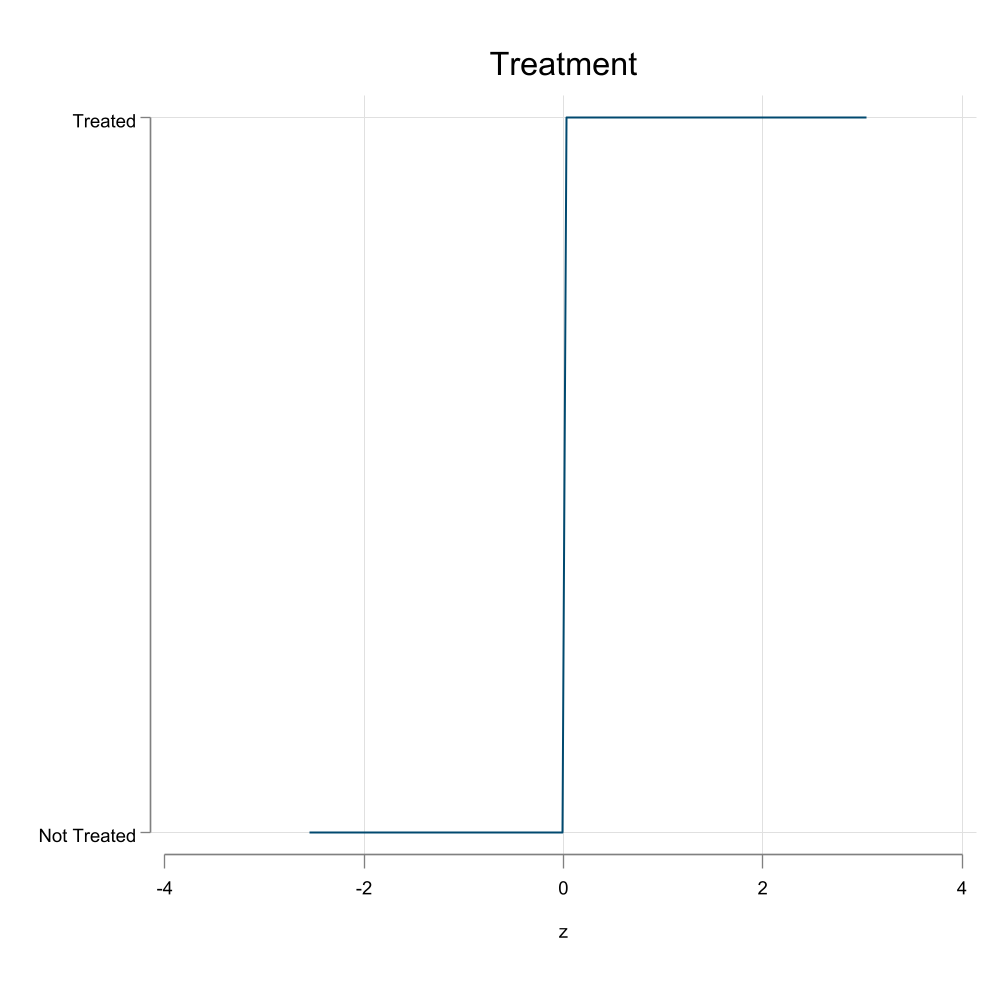
\includegraphics{resources/rdd1.png}

}

\end{minipage}%
%
\begin{minipage}[t]{0.50\linewidth}

\raisebox{-\height}{

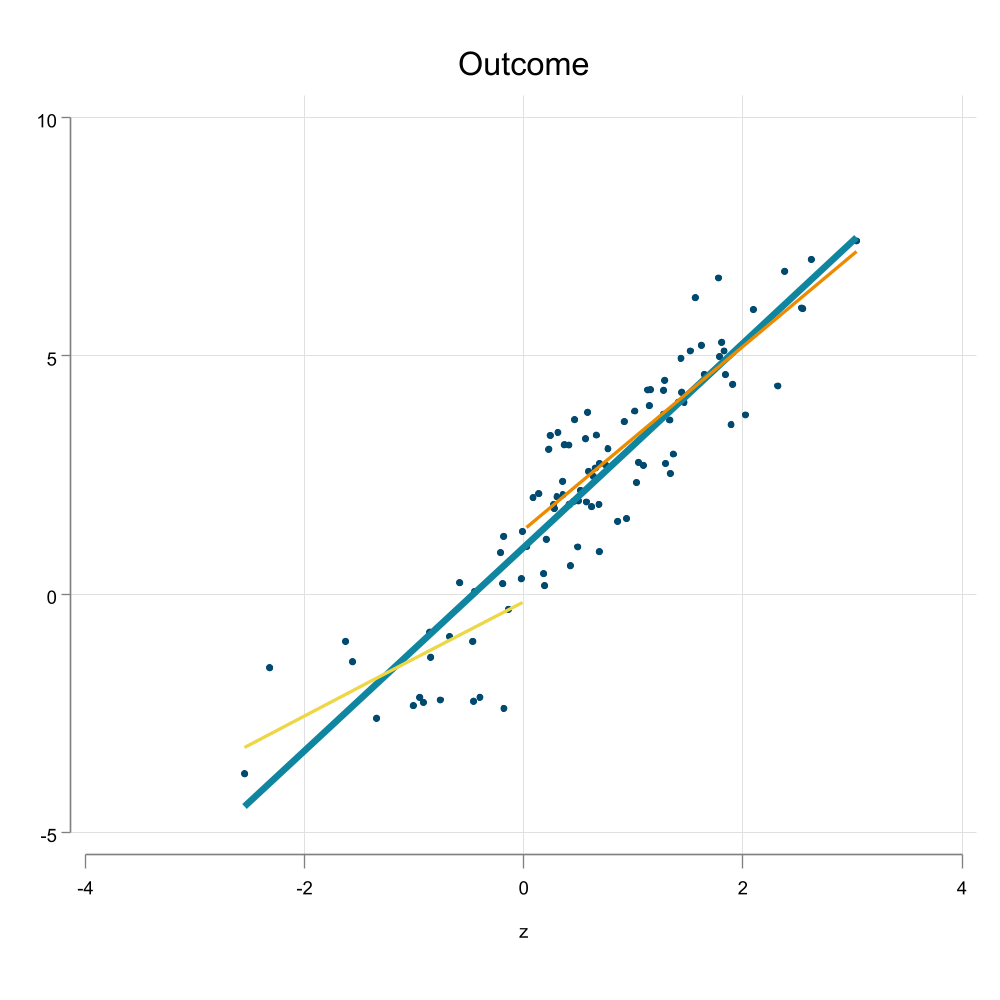
\includegraphics{resources/rdd2.png}

}

\end{minipage}%

\end{figure}%

\subsection{How it works : p2}\label{how-it-works-p2}

Recall that in an RCT (or under randomization) treatment effects are
estimated by comparing those treated and those not treated.

\[E(y|D=1)-E(y|D=0)\]

Under SRDD, you can also think about the same experiment, except that we
would need to compare individuals AT the theshold.

\[\begin{aligned}
\lim_{z\downarrow c} E(y|Z=z) &- \lim_{z\uparrow c} E(y|Z=z) \\
E(y(1)|Z=c) &-E(y(0)|Z=c)
\end{aligned}
\]

\begin{itemize}
\tightlist
\item
  In this case, the overlapping assumption is violated. So we need to
  attemp obtaining effects for groups AT the limit when \(Z=c\).
\end{itemize}

\subsection{Estimation}\label{estimation}

The most simple way to proceed is to estimate the model using a
parametric approach (OLS)

\[y = a_0 + \delta D_{z>c} + f(z-c) + e\]

The idea here is to identify a ``jump'' in the outcome (treatment
effect) at the point where \(z\) crosses the threshold.

But to identify the jump only, we also need to model the trend observe
before and after that threshold (\(f(z-c)\)), which can be modelled as
flexible as possible. (this include interactions with the jump)

Alternatively, we could use smaller bandwidths (nonparametric)

\subsection{Example}\label{example}

\begin{Shaded}
\begin{Highlighting}[]
 \KeywordTok{qui}\NormalTok{: \{}
\KeywordTok{clear}
\KeywordTok{set} \DecValTok{seed}\NormalTok{ 1}
\KeywordTok{set} \KeywordTok{obs}\NormalTok{ 200}
\KeywordTok{gen} \FunctionTok{e}\NormalTok{=rnormal()}
\KeywordTok{gen}\NormalTok{ z=runiform()+}\FunctionTok{e}
\KeywordTok{sum}\NormalTok{ z}
\KeywordTok{replace}\NormalTok{ z=(z{-}}\FunctionTok{r}\NormalTok{(}\KeywordTok{mean}\NormalTok{))/}\FunctionTok{r}\NormalTok{(}\FunctionTok{sd}\NormalTok{)}
\KeywordTok{gen}\NormalTok{ t = z\textgreater{}0}
\KeywordTok{gen} \FunctionTok{y}\NormalTok{ = 1 + 0.5*z + }\FunctionTok{e}\NormalTok{ + rnormal() + (z\textgreater{}0)}

\KeywordTok{qui}\NormalTok{:}\KeywordTok{reg} \FunctionTok{y}\NormalTok{ t z }
\KeywordTok{predict}\NormalTok{ yh1}
\KeywordTok{local}\NormalTok{ b1:}\KeywordTok{display}\NormalTok{ \%3.2f \_b[t]}
\KeywordTok{qui}\NormalTok{:}\KeywordTok{reg} \FunctionTok{y}\NormalTok{ t c.z\#\#c.z  }
\KeywordTok{predict}\NormalTok{ yh2}
\KeywordTok{local}\NormalTok{ b2:}\KeywordTok{display}\NormalTok{ \%3.2f \_b[t]}
\KeywordTok{qui}\NormalTok{:}\KeywordTok{reg} \FunctionTok{y}\NormalTok{ t c.z\#\#c.z\#\#c.z}
\KeywordTok{predict}\NormalTok{ yh3}
\KeywordTok{local}\NormalTok{ b3:}\KeywordTok{display}\NormalTok{ \%3.2f \_b[t]}
\KeywordTok{sort}\NormalTok{ z}
\NormalTok{\}}
\KeywordTok{two}\NormalTok{ (}\KeywordTok{scatter} \FunctionTok{y}\NormalTok{ z, }\KeywordTok{sort} \BaseNTok{title}\NormalTok{(}\StringTok{"Sharp RDD"}\NormalTok{) pstyle(p1) }\KeywordTok{color}\NormalTok{(\%20)) }\CommentTok{///}
\NormalTok{    (}\KeywordTok{line}\NormalTok{ yh1 z }\KeywordTok{if}\NormalTok{ z\textless{}0, pstyle(p2) lw(0.5)) (}\KeywordTok{line}\NormalTok{ yh1 z }\KeywordTok{if}\NormalTok{ z\textgreater{}0, pstyle(p2) lw(0.5)) }\CommentTok{///}
\NormalTok{    (}\KeywordTok{line}\NormalTok{ yh2 z }\KeywordTok{if}\NormalTok{ z\textless{}0, pstyle(p3) lw(0.5)) (}\KeywordTok{line}\NormalTok{ yh2 z }\KeywordTok{if}\NormalTok{ z\textgreater{}0, pstyle(p3) lw(0.5)) }\CommentTok{///}
\NormalTok{    (}\KeywordTok{line}\NormalTok{ yh3 z }\KeywordTok{if}\NormalTok{ z\textless{}0, pstyle(p4) lw(0.5)) (}\KeywordTok{line}\NormalTok{ yh3 z }\KeywordTok{if}\NormalTok{ z\textgreater{}0, pstyle(p4) lw(0.5)) , }\CommentTok{///}
    \BaseNTok{legend}\NormalTok{(}\KeywordTok{order}\NormalTok{(2 }\StringTok{"Linear ATT: \textasciigrave{}b1\textquotesingle{}"}\NormalTok{ 3 }\StringTok{"Quadratic ATT: \textasciigrave{}b2\textquotesingle{}"}\NormalTok{ 4 }\StringTok{"Cubic ATT: \textasciigrave{}b3\textquotesingle{}"}\NormalTok{)) }\BaseNTok{name}\NormalTok{(m1, }\KeywordTok{replace}\NormalTok{)}
\end{Highlighting}
\end{Shaded}

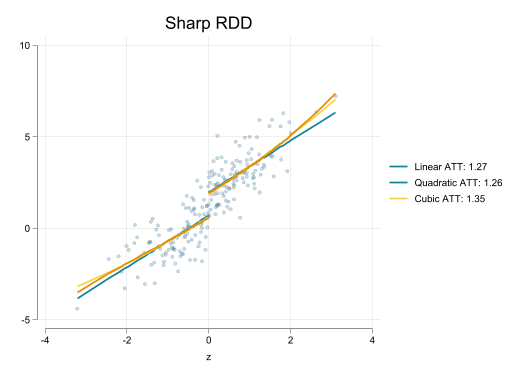
\includegraphics{11rdd_files/figure-pdf/cell-3-output-1.png}

\subsection{Example}\label{example-1}

\begin{Shaded}
\begin{Highlighting}[]
\KeywordTok{qui}\NormalTok{: \{}
\KeywordTok{qui}\NormalTok{:}\KeywordTok{reg} \FunctionTok{y}\NormalTok{ t c.z\#t }
\KeywordTok{predict}\NormalTok{ yh11}
\KeywordTok{local}\NormalTok{ b1:}\KeywordTok{display}\NormalTok{ \%3.2f \_b[t]}
\KeywordTok{qui}\NormalTok{:}\KeywordTok{reg} \FunctionTok{y}\NormalTok{ t (c.z\#\#c.z)\#t  }
\KeywordTok{predict}\NormalTok{ yh21}
\KeywordTok{local}\NormalTok{ b2:}\KeywordTok{display}\NormalTok{ \%3.2f \_b[t]}
\KeywordTok{qui}\NormalTok{:}\KeywordTok{reg} \FunctionTok{y}\NormalTok{ t (c.z\#\#c.z\#\#c.z)\#t}
\KeywordTok{predict}\NormalTok{ yh31}
\KeywordTok{local}\NormalTok{ b3:}\KeywordTok{display}\NormalTok{ \%3.2f \_b[t]}
\NormalTok{\}}
\KeywordTok{two}\NormalTok{ (}\KeywordTok{scatter} \FunctionTok{y}\NormalTok{ z, }\KeywordTok{sort} \BaseNTok{title}\NormalTok{(}\StringTok{"Sharp RDD"}\NormalTok{) pstyle(p1) }\KeywordTok{color}\NormalTok{(\%20)) }\CommentTok{///}
\NormalTok{    (}\KeywordTok{line}\NormalTok{ yh11 z }\KeywordTok{if}\NormalTok{ z\textless{}0, pstyle(p2) lw(0.5)) (}\KeywordTok{line}\NormalTok{ yh11 z }\KeywordTok{if}\NormalTok{ z\textgreater{}0, pstyle(p2) lw(0.5)) }\CommentTok{///}
\NormalTok{    (}\KeywordTok{line}\NormalTok{ yh21 z }\KeywordTok{if}\NormalTok{ z\textless{}0, pstyle(p3) lw(0.5)) (}\KeywordTok{line}\NormalTok{ yh21 z }\KeywordTok{if}\NormalTok{ z\textgreater{}0, pstyle(p3) lw(0.5)) }\CommentTok{///}
\NormalTok{    (}\KeywordTok{line}\NormalTok{ yh31 z }\KeywordTok{if}\NormalTok{ z\textless{}0, pstyle(p4) lw(0.5)) (}\KeywordTok{line}\NormalTok{ yh31 z }\KeywordTok{if}\NormalTok{ z\textgreater{}0, pstyle(p4) lw(0.5)) , }\CommentTok{///}
    \BaseNTok{legend}\NormalTok{(}\KeywordTok{order}\NormalTok{(2 }\StringTok{"Linear ATT: \textasciigrave{}b1\textquotesingle{}"}\NormalTok{ 3 }\StringTok{"Quadratic ATT: \textasciigrave{}b2\textquotesingle{}"}\NormalTok{ 4 }\StringTok{"Cubic ATT: \textasciigrave{}b3\textquotesingle{}"}\NormalTok{)) }\BaseNTok{name}\NormalTok{(m2, }\KeywordTok{replace}\NormalTok{) }
\end{Highlighting}
\end{Shaded}

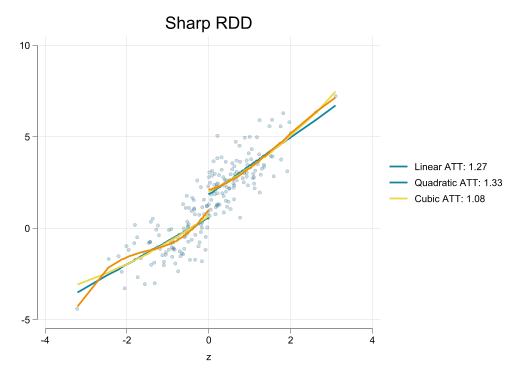
\includegraphics{11rdd_files/figure-pdf/cell-4-output-1.png}

\subsection{Fuzzy RD: Imperfect
compliance}\label{fuzzy-rd-imperfect-compliance}

While the Idea Scenario happens when there is perfect compliance (above
the threshold you are treated), this doesnt happen all the time.

In the education example:

\begin{itemize}
\tightlist
\item
  Some people with low grades may be ``legacy'' or have ``contacts'' (or
  took a second exam later) and manage to go to college
\item
  Some decided not to go, even after entering to college
\end{itemize}

Sounds Familiar? (Never takers vs always takers)

When this happens, you can still do RDD, but you need more steps

\subsection{Fuzzy RD}\label{fuzzy-rd}

\begin{enumerate}
\def\labelenumi{\arabic{enumi}.}
\tightlist
\item
  Estimate the impact of Discontinuity on Treatment
\item
  Estimate the impact of Discontinuity on Outcome
\item
  Estimate the ratio between (1) and (2)
\end{enumerate}

Sounds Familiar?

\begin{itemize}
\tightlist
\item
  Its a kind of wald/IV estimator.

  \begin{itemize}
  \tightlist
  \item
    The instrument is the discontinuity
  \item
    The the endogenous variable is the treament
  \end{itemize}
\end{itemize}

You still need to estimate the effect as close to the Discontinuity as
possible

\texttt{ivregress} may still do most of this for you

\subsection{Example}\label{example-2}

\begin{figure}

\begin{minipage}[t]{0.50\linewidth}

\begin{figure}

{\centering 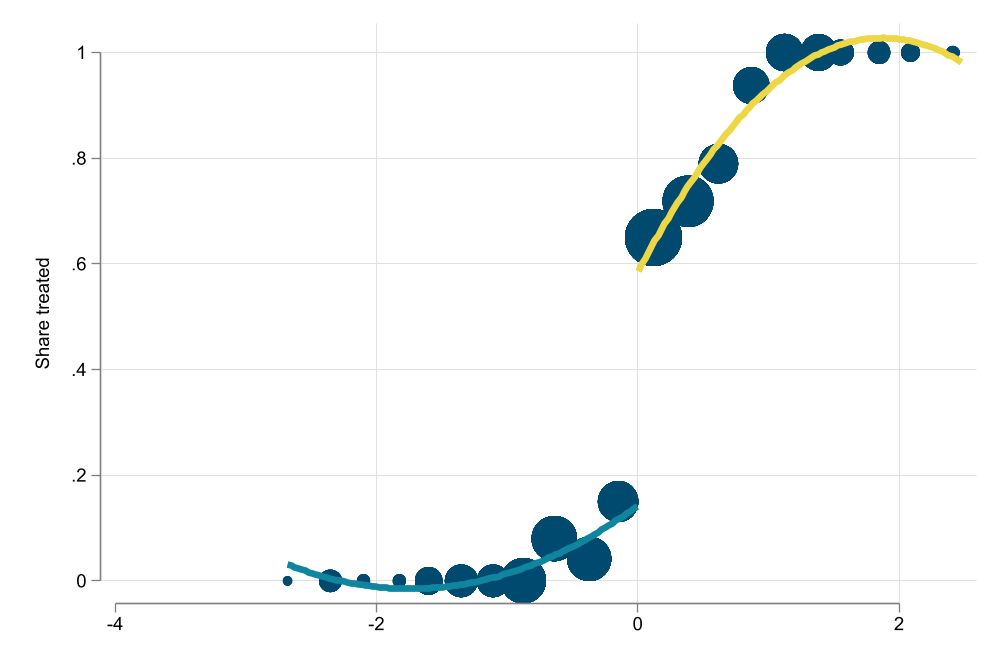
\includegraphics{resources/frdd1.png}

}
\caption{Treatment}

\end{figure}%

\end{minipage}%
%
\begin{minipage}[t]{0.50\linewidth}

\begin{figure}

{\centering 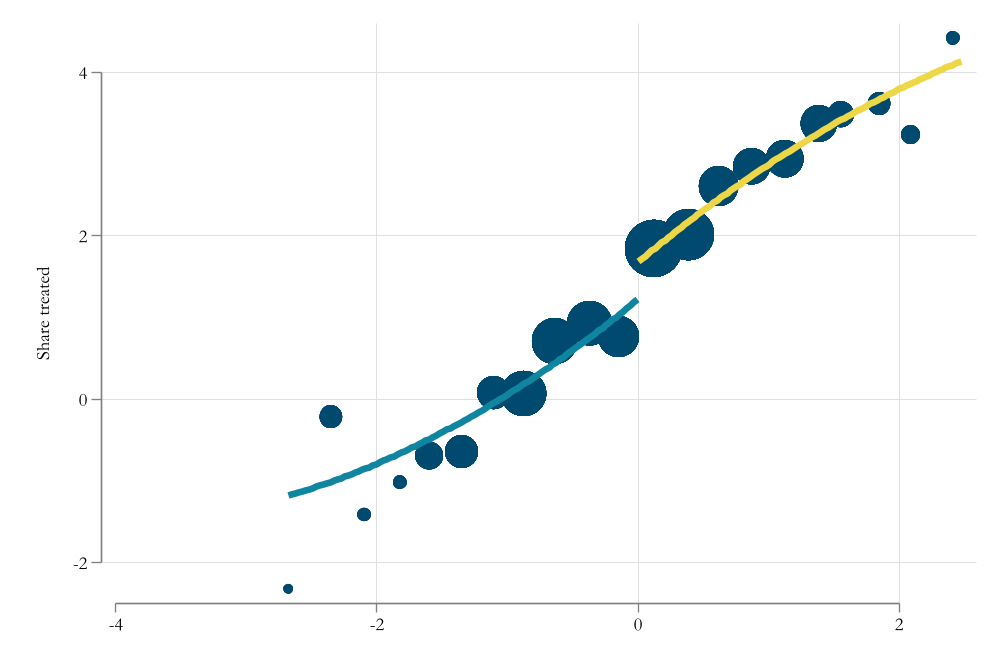
\includegraphics{resources/frdd2.png}

}
\caption{Outcome}

\end{figure}%

\end{minipage}%

\end{figure}%

Effect:

\begin{Shaded}
\begin{Highlighting}[]
\KeywordTok{qui}\NormalTok{: }\KeywordTok{gen}\NormalTok{ dz = z\textgreater{}0}
\KeywordTok{qui}\NormalTok{: }\KeywordTok{reg} \FunctionTok{y}\NormalTok{ dz c.z\#\#c.z\#i.dz}
\KeywordTok{local}\NormalTok{ b1 = \_b[dz]}
\KeywordTok{qui}\NormalTok{: }\KeywordTok{reg}\NormalTok{ t dz c.z\#\#c.z\#i.dz}
\KeywordTok{local}\NormalTok{ b2 = \_b[dz]}

\KeywordTok{display} \StringTok{"There is a "}\NormalTok{ \%3.2f }\OtherTok{\textasciigrave{}b1\textquotesingle{}} \StringTok{" effect on the outcome"}
\KeywordTok{display} \StringTok{"and a "}\NormalTok{ \%3.2f }\OtherTok{\textasciigrave{}b2\textquotesingle{}} \StringTok{" effect on the treatment"}
\KeywordTok{display} \StringTok{"which imply a LATE of "}\NormalTok{ \%3.2f }\OtherTok{\textasciigrave{}=\textasciigrave{}b1\textquotesingle{}}\NormalTok{/}\OtherTok{\textasciigrave{}b2\textquotesingle{}}\NormalTok{\textquotesingle{}}
\end{Highlighting}
\end{Shaded}

There is a 0.45 effect on the outcome and a 0.44 effect on the treatment
which imply a LATE of 1.03

\subsection{Things to consider}\label{things-to-consider}

\textbf{Theoretical}:

\begin{enumerate}
\def\labelenumi{\arabic{enumi}.}
\tightlist
\item
  You need to identify ``jumps'' caused by a running variable. (depends
  on knowing how things works)
\item
  The potential outcomes have to be smooth functions of the running
  variable
\end{enumerate}

\textbf{Empirical}:

\begin{enumerate}
\def\labelenumi{\arabic{enumi}.}
\setcounter{enumi}{2}
\tightlist
\item
  The running variable shouldnt be manipulated. (random)

  \begin{itemize}
  \tightlist
  \item
    Implies Assignment rules are not known, are exogenous, and there is
    no random heaping
  \end{itemize}
\item
  Controls should be balanced around the threshold
\end{enumerate}

\subsection{Testing Empirical
Assumptions}\label{testing-empirical-assumptions}

Manipulation of running variable may cause a non-smooth density in the
running variable:

\begin{itemize}
\tightlist
\item
  If there is no manipulation, you may expect density round threshold to
  be smooth.

  \begin{itemize}
  \tightlist
  \item
    In Stata: ssc install \texttt{rddensity}. In r
    install.packages(c(`rdd',`rddensity'))
  \end{itemize}
\end{itemize}

\begin{Shaded}
\begin{Highlighting}[]
\KeywordTok{set} \DecValTok{linesize}\NormalTok{ 100}
\KeywordTok{qui}\NormalTok{:}\KeywordTok{ssc}\NormalTok{ install  lpdensity, }\KeywordTok{replace}
\KeywordTok{qui}\NormalTok{:}\KeywordTok{ssc}\NormalTok{ install  rddensity, }\KeywordTok{replace}
\NormalTok{rddensity z, c(0) plot}
\KeywordTok{graph} \KeywordTok{export}\NormalTok{ resources\textbackslash{}frdd3.png, }\KeywordTok{width}\NormalTok{(1000) }\KeywordTok{replace}
\end{Highlighting}
\end{Shaded}

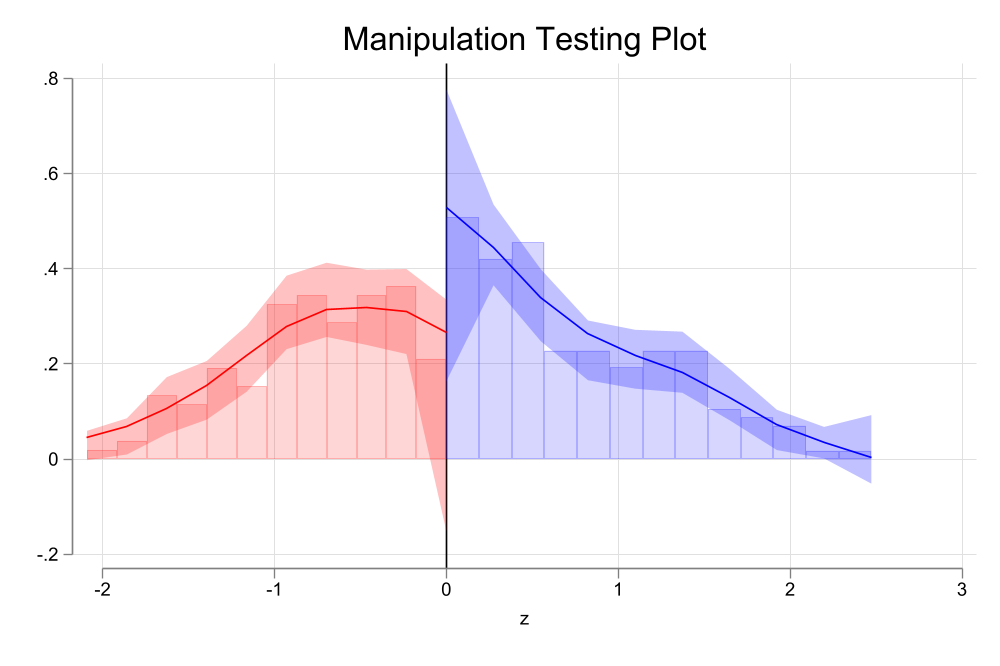
\includegraphics{resources/frdd3.png}

\subsection{}\label{section-2}

\begin{itemize}
\item
  In cases of nonrandom heaping, it may be possible to avoid the problem
  by restricting the data.
\item
  This is an example of measurement error, when individuals may
  ``round-up/down'' answers. And may occure near threshold.
\item
  This does not necessarily mean there is manipulation.
\item
  Possible Solution? Estimate RDD excluding observations around
  (excluding) threshold.
\end{itemize}

\subsection{Covariate balance and Placebo
tests}\label{covariate-balance-and-placebo-tests}

\begin{itemize}
\item
  If treatment is \textbf{locally} randomized, then covariates should
  not be affected by discontinuity.
\item
  Alternatively, one could estimate effects on variables you know CANNOT
  be affected by the treatment
\item
  One could also implement a placebo test, checking the impact on a
  different threholds.

  \begin{itemize}
  \tightlist
  \item
    No effect should be observed on the outcome, (but some on the
    treatment)
  \end{itemize}
\end{itemize}

\subsection{Example}\label{example-3}

Impact of Scores on Scholarship recipiency

\begin{Shaded}
\begin{Highlighting}[]
\KeywordTok{use}\NormalTok{ resources\textbackslash{}fuzzy, }\KeywordTok{clear}
\NormalTok{color\_style bay}
\KeywordTok{qui}\NormalTok{:rdplot }\KeywordTok{d}\NormalTok{ x1, graph\_options(}\BaseNTok{legend}\NormalTok{( pos(6)))}
\end{Highlighting}
\end{Shaded}

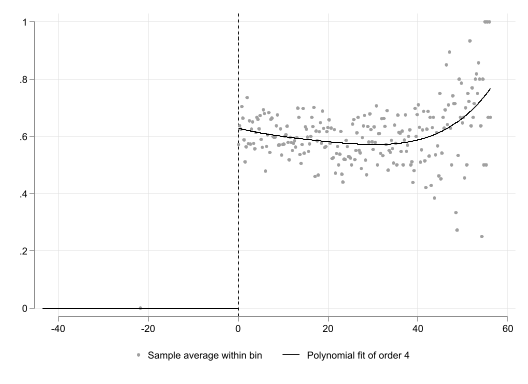
\includegraphics{11rdd_files/figure-pdf/cell-8-output-1.png}

\subsection{Manipulation test}\label{manipulation-test}

\begin{Shaded}
\begin{Highlighting}[]
\KeywordTok{qui}\NormalTok{:rddensity x1, plot}
\end{Highlighting}
\end{Shaded}

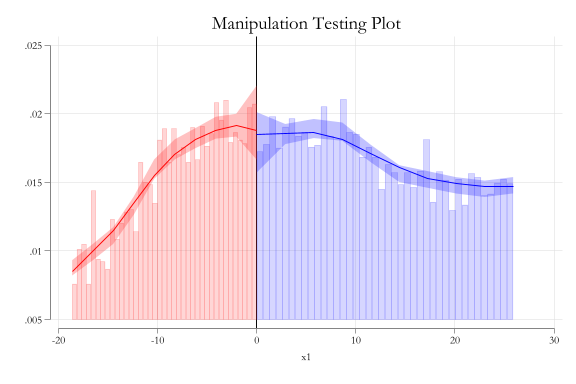
\includegraphics{11rdd_files/figure-pdf/cell-9-output-1.png}

\subsection{Intention to treat}\label{intention-to-treat}

Impact on Enrollment

\begin{Shaded}
\begin{Highlighting}[]
\KeywordTok{qui}\NormalTok{:rdplot }\FunctionTok{y}\NormalTok{ x1, graph\_options(}\BaseNTok{legend}\NormalTok{( pos(6)))}
\end{Highlighting}
\end{Shaded}

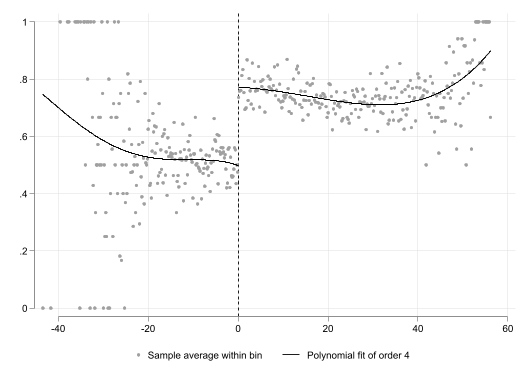
\includegraphics{11rdd_files/figure-pdf/cell-10-output-1.png}

\subsection{Estimation of the effect:}\label{estimation-of-the-effect}

\begin{Shaded}
\begin{Highlighting}[]
\KeywordTok{gen}\NormalTok{ dx1 = x1\textgreater{}0}
\NormalTok{ivregress 2sls }\FunctionTok{y}\NormalTok{ (}\KeywordTok{d}\NormalTok{ = dx1) c.x1\#\#c.x1\#dx1 }
\end{Highlighting}
\end{Shaded}

\begin{verbatim}

Instrumental variables 2SLS regression            Number of obs   =     23,132
                                                  Wald chi2(5)    =    1645.56
                                                  Prob > chi2     =     0.0000
                                                  R-squared       =     0.2845
                                                  Root MSE        =     .39876

-------------------------------------------------------------------------------
            y | Coefficient  Std. err.      z    P>|z|     [95% conf. interval]
--------------+----------------------------------------------------------------
            d |   .4432824   .0215111    20.61   0.000     .4011214    .4854434
              |
     dx1#c.x1 |
           0  |   .0002949   .0019179     0.15   0.878    -.0034642    .0040539
           1  |  -.0034238    .000779    -4.39   0.000    -.0049507   -.0018969
              |
dx1#c.x1#c.x1 |
           0  |   .0000741   .0000703     1.05   0.292    -.0000637    .0002119
           1  |   .0000616   .0000164     3.76   0.000     .0000295    .0000936
              |
        _cons |   .5103635    .010876    46.93   0.000     .4890469    .5316801
-------------------------------------------------------------------------------
Instrumented: d
 Instruments: 0b.dx1#c.x1 1.dx1#c.x1 0b.dx1#c.x1#c.x1 1.dx1#c.x1#c.x1 dx1
\end{verbatim}

\subsection{Some Sensitivity}\label{some-sensitivity}

\begin{Shaded}
\begin{Highlighting}[]
\KeywordTok{qui}\NormalTok{:\{   }
\FunctionTok{matrix}\NormalTok{ b1 = 0,0}
\KeywordTok{forvalues}\NormalTok{ i = 1/15 \{}
\NormalTok{    ivregress 2sls }\FunctionTok{y}\NormalTok{ (}\KeywordTok{d}\NormalTok{ = dx1) c.x1\#dx1  }\KeywordTok{if} \FunctionTok{abs}\NormalTok{(x1)\textless{}}\OtherTok{\textasciigrave{}i\textquotesingle{}}
    \FunctionTok{matrix}\NormalTok{ b1=b1\textbackslash{}[\_b[}\KeywordTok{d}\NormalTok{],\_se[}\KeywordTok{d}\NormalTok{]]}
\NormalTok{\}}

\FunctionTok{matrix}\NormalTok{ b2 = 0,0}
\KeywordTok{forvalues}\NormalTok{ i = 1/15 \{}
\NormalTok{    ivregress 2sls }\FunctionTok{y}\NormalTok{ (}\KeywordTok{d}\NormalTok{ = dx1) c.x1\#\#c.x1\#dx1  }\KeywordTok{if} \FunctionTok{abs}\NormalTok{(x1)\textless{}}\OtherTok{\textasciigrave{}i\textquotesingle{}}
    \FunctionTok{matrix}\NormalTok{ b2=b2\textbackslash{}[\_b[}\KeywordTok{d}\NormalTok{],\_se[}\KeywordTok{d}\NormalTok{]]}
\NormalTok{\}}

\FunctionTok{matrix}\NormalTok{ b3 = 0,0}
\KeywordTok{forvalues}\NormalTok{ i = 1/15 \{}
\NormalTok{    ivregress 2sls }\FunctionTok{y}\NormalTok{ (}\KeywordTok{d}\NormalTok{ = dx1) c.x1\#\#c.x1\#\#c.x1\#dx1  }\KeywordTok{if} \FunctionTok{abs}\NormalTok{(x1)\textless{}}\OtherTok{\textasciigrave{}i\textquotesingle{}}
    \FunctionTok{matrix}\NormalTok{ b3=b3\textbackslash{}[\_b[}\KeywordTok{d}\NormalTok{],\_se[}\KeywordTok{d}\NormalTok{]]}
\NormalTok{\}}

\NormalTok{lbsvmat b1}
\NormalTok{lbsvmat b2}
\NormalTok{lbsvmat b3}
\KeywordTok{forvalues}\NormalTok{ i = 1/3 \{}
  \KeywordTok{gen}\NormalTok{ ll}\OtherTok{\textasciigrave{}i\textquotesingle{}}\NormalTok{=b}\OtherTok{\textasciigrave{}i\textquotesingle{}}\NormalTok{1{-}b}\OtherTok{\textasciigrave{}i\textquotesingle{}}\NormalTok{2*1.96}
  \KeywordTok{gen}\NormalTok{ ul}\OtherTok{\textasciigrave{}i\textquotesingle{}}\NormalTok{=b}\OtherTok{\textasciigrave{}i\textquotesingle{}}\NormalTok{1+b}\OtherTok{\textasciigrave{}i\textquotesingle{}}\NormalTok{2*1.96}
\NormalTok{\}}
\KeywordTok{gen}\NormalTok{ z = }\DataTypeTok{\_n}\NormalTok{{-}1 }\KeywordTok{if}\NormalTok{ b11!=.}
\KeywordTok{replace}\NormalTok{ z=. }\KeywordTok{in}\NormalTok{ 1}

\NormalTok{\}}
\KeywordTok{gen}\NormalTok{ z1 = z + 0.25}
\KeywordTok{gen}\NormalTok{ z2 = z + 0.5}
\KeywordTok{two}\NormalTok{ (rspike ll1 ul1 z, lw(1) pstyle(p1) }\KeywordTok{color}\NormalTok{(\%50) ) (}\KeywordTok{scatter}\NormalTok{ b11 z, pstyle(p1) ) }\CommentTok{///}
\NormalTok{    (rspike ll2 ul2 z1, lw(1) pstyle(p2) }\KeywordTok{color}\NormalTok{(\%50) ) (}\KeywordTok{scatter}\NormalTok{ b21 z1, pstyle(p2) ) }\CommentTok{///}
\NormalTok{    (rspike ll3 ul3 z2, lw(1) pstyle(p3) }\KeywordTok{color}\NormalTok{(\%50) ) (}\KeywordTok{scatter}\NormalTok{ b31 z2, pstyle(p3) ), }\CommentTok{///}
    \BaseNTok{legend}\NormalTok{(}\KeywordTok{order}\NormalTok{(1 }\StringTok{"Linear"}\NormalTok{ 3 }\StringTok{"Quadratic"}\NormalTok{ 5 }\StringTok{"Cubic"}\NormalTok{)) }\BaseNTok{xtitle}\NormalTok{(}\StringTok{"Bandwidth"}\NormalTok{)}
\end{Highlighting}
\end{Shaded}

\begin{verbatim}
(23,117 missing values generated)
(23,117 missing values generated)
\end{verbatim}

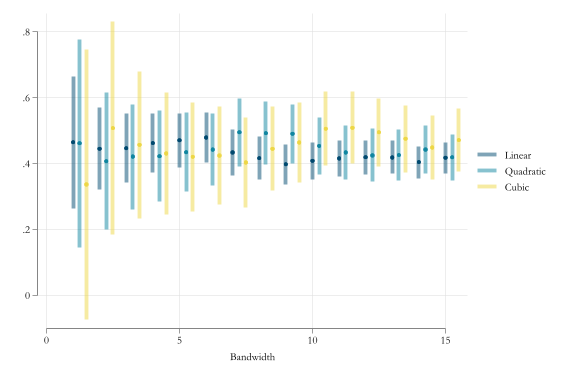
\includegraphics{11rdd_files/figure-pdf/cell-12-output-2.png}

\subsection{Flasification test}\label{flasification-test}

\begin{Shaded}
\begin{Highlighting}[]
\KeywordTok{qui}\NormalTok{ \{}
\NormalTok{ivregress 2sls icfes\_female (}\KeywordTok{d}\NormalTok{ = dx1) c.x1\#dx1    }\KeywordTok{if} \FunctionTok{abs}\NormalTok{(x1)\textless{}20}
\KeywordTok{est}\NormalTok{ sto m1}
\NormalTok{ivregress 2sls icfes\_age (}\KeywordTok{d}\NormalTok{ = dx1) c.x1\#dx1       }\KeywordTok{if} \FunctionTok{abs}\NormalTok{(x1)\textless{}20}
\KeywordTok{est}\NormalTok{ sto m2}
\NormalTok{ivregress 2sls icfes\_urm (}\KeywordTok{d}\NormalTok{ = dx1) c.x1\#dx1       }\KeywordTok{if} \FunctionTok{abs}\NormalTok{(x1)\textless{}20}
\KeywordTok{est}\NormalTok{ sto m3}
\NormalTok{ivregress 2sls icfes\_famsize (}\KeywordTok{d}\NormalTok{ = dx1) c.x1\#dx1       }\KeywordTok{if} \FunctionTok{abs}\NormalTok{(x1)\textless{}20}
\KeywordTok{est}\NormalTok{ sto m4}
\NormalTok{\}}
\NormalTok{esttab m1 m2 m3 m4, }\KeywordTok{keep}\NormalTok{(}\KeywordTok{d}\NormalTok{)}
\end{Highlighting}
\end{Shaded}

\begin{verbatim}

----------------------------------------------------------------------------
                      (1)             (2)             (3)             (4)   
             icfes_female       icfes_age       icfes_urm    icfes_fams~e   
----------------------------------------------------------------------------
d                  0.0199           0.128         0.00791          0.0439   
                   (0.80)          (1.05)          (0.65)          (0.63)   
----------------------------------------------------------------------------
N                   14841           14799           14841           14801   
----------------------------------------------------------------------------
t statistics in parentheses
* p<0.05, ** p<0.01, *** p<0.001
\end{verbatim}

\section{Next Differences in
Differences}\label{next-differences-in-differences}



\end{document}
